\section{Bayesian Calibration}
\label{sec:bayes}

As discussed earlier in Section~\ref{sec:intro}, the underlying methodology for determining the nominal 
estimates for SW potential parameters did not account for measurement error, inadequate functional
form of the potential, inherent noise in MD predictions, and parametric uncertainties. Hence, there is
a possibility of improving the estimates since using the same set of values for a wide variety of systems
and applications is not ideal. A robust approach to calibrating the parameters in the presence of
such uncertainties is made possible by using a Bayesian framework. The methodology aims at evaluating
the so-called joint posterior probability distribution (referred to as the `posterior') of the uncertain model 
parameters to be calibrated, using the Bayes' rule:

\be
\mathcal{P}(\bm{X}\vert \bm{Y}) \propto \mathcal{P}(\bm{Y}\vert\bm{X})\mathcal{P}(\bm{X})
\ee

\noindent where $\bm{X}$ is the set of uncertain model parameters, and $\bm{Y}$ is the available set of
experimental data i.e. bulk thermal conductivity at different temperatures in the present case. 
We exploit our findings based on sensitivity analysis in
Figure~\ref{fig:gsa} and focus on calibrating $\alpha$ and $\gamma$ i.e. $\bm{X}:\{\alpha,\gamma\}$.
$\mathcal{P}(\bm{X}\vert \bm{Y})$ is regarded as the posterior, $\mathcal{P}(\bm{Y}\vert\bm{X})$ is the
`likelihood', and $\mathcal{P}(\bm{X})$ is the joint prior probability distribution (referred to as the `prior') of $\bm{X}$.
The likelihood accounts for measurement error, and the discrepancy between experiments and model
predictions, whereas, the prior is an initial guess for the distribution of uncertain model parameters in an
interval. It also accounts for the availability of an expert opinion pertaining to their estimates. 
The posterior provides an estimate of the most likely value of the uncertain model parameters based on
prior uncertainty, experimental data used for calibration and the associated measurement error, and model
discrepancy. Additionally, the posterior is often used to quantify the uncertainty associated with model predictions. Several algorithms based on Markov chain Monte Carlo (MCMC) technique are available for  
sampling the posterior~\cite{Haario:2001, Haario:2006,Xu:2014}.

Evaluating the joint posterior of $\alpha$ and $\gamma$ using MCMC typically requires a large amount of
computational effort and is not the focus on this work. Instead, we compute and plot the joint likelihood on
a 2D cartesian grid described by $\alpha$ and $\gamma$ using Eq.~\ref{eq:like} as illustrated in
Figure~\ref{fig:like}(a). For this purpose, we consider $\alpha$ and $\gamma$ to be
independent and uniformly distributed in the intervals, [1.62,1.98] and [1.08,1.32] respectively. 
Consequently, the posterior is proportional to the likelihood, considered to be a Gaussian:

\be
\mathcal{P}(\bm{Y}\vert\bm{X}) = \frac{1}{\sqrt{2\pi\sigma^2}}\exp\left[-\frac{(\kappa_{\tiny{\mbox{E}}} - 
\kappa_{\tiny{\mbox{MD}}})^2}{2\sigma^2}\right]
\label{eq:like}
\ee

\noindent where $\sigma$ is the standard deviation of the measurement error, and
$(\kappa_{\tiny{\mbox{E}}} - \kappa_{\tiny{\mbox{MD}}})$ is the discrepancy between 
NEMD predictions~($\kappa_{\tiny{\mbox{MD}}}$)
and experimental data~($\kappa_{\tiny{\mbox{E}}}$). Experimental data for $\kappa_{\tiny{\mbox{E}}}$ at 300~K
(149~W/m/K~\cite{Shanks:1963}) is used to compute the joint likelihood. 

\begin{figure}[htbp]
 \begin{center}
  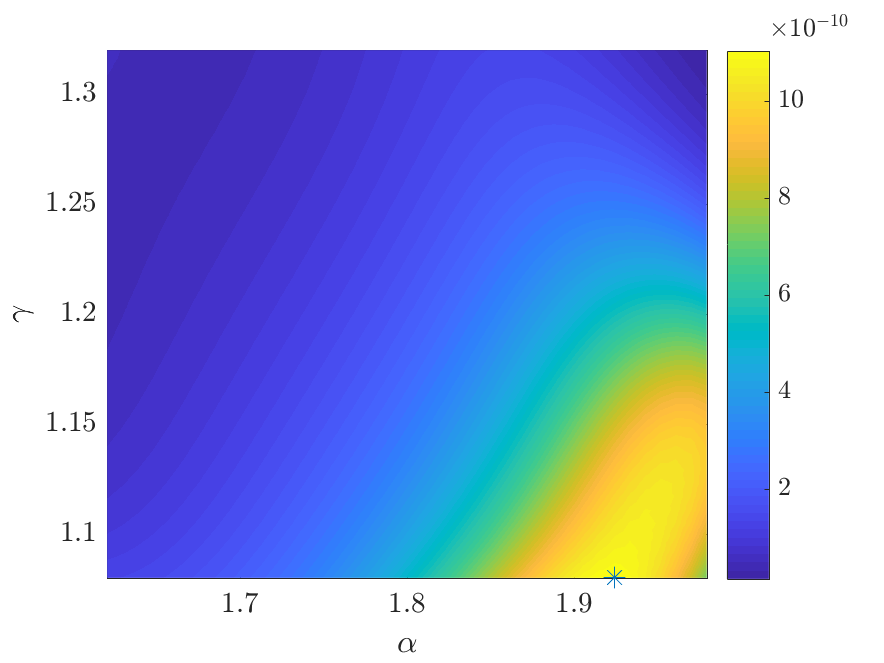
\includegraphics[width=0.70\textwidth]{./Figures/gl}
  \\ (a)
  \begin{tabular}{cc}
  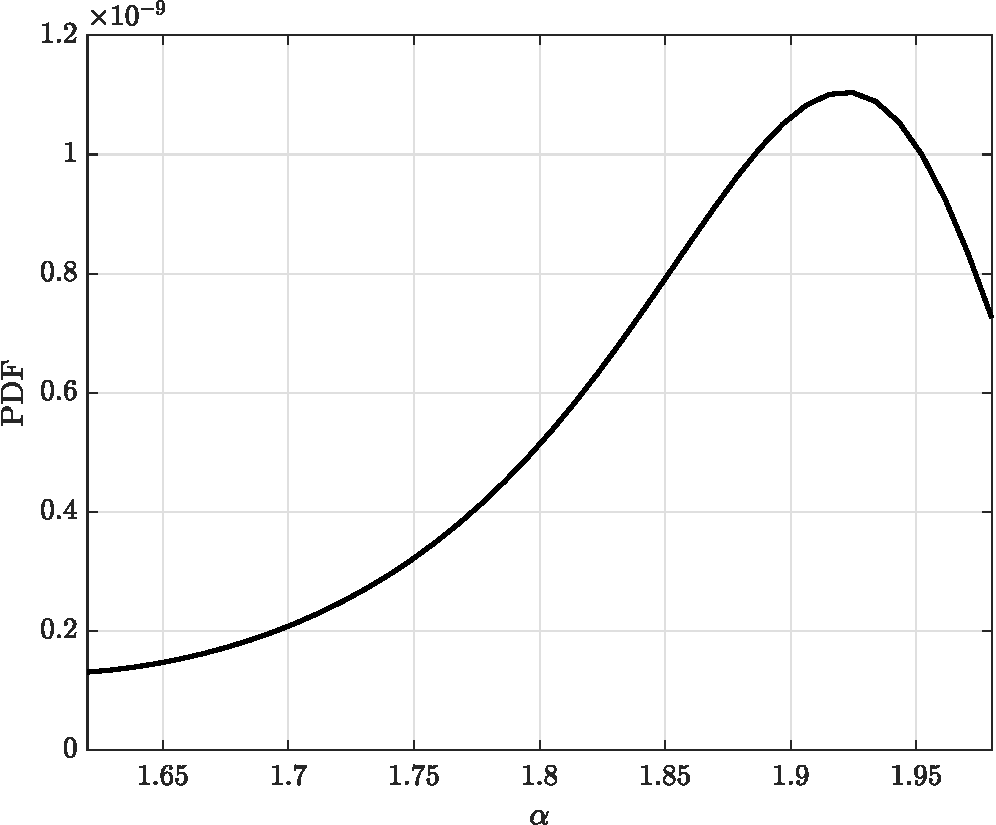
\includegraphics[width=0.50\textwidth]{./Figures/pdf_alpha}
  &
  %\hspace{3mm}
  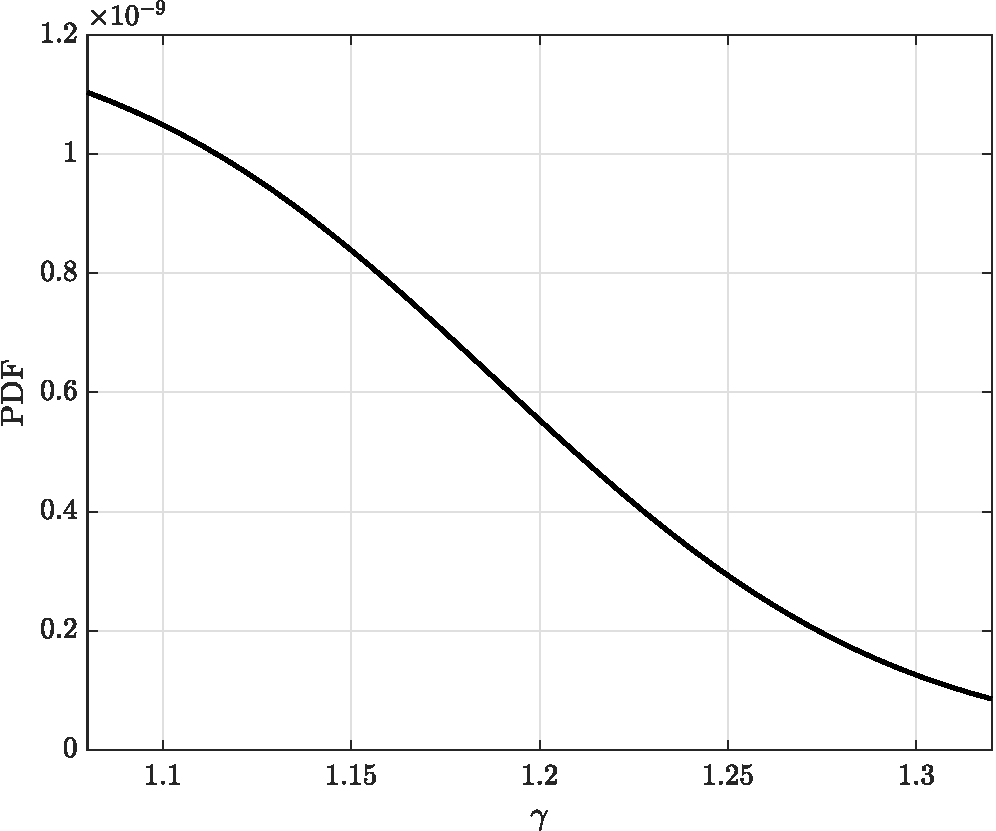
\includegraphics[width=0.50\textwidth]{./Figures/pdf_gamma}
  \\ (b) & (c)
  \end{tabular}
\caption{(a) A joint likelihood as estimated using Eq.~\ref{eq:like} is plotted on a 2D cartesian grid
 ($\alpha\times\gamma$). Point corresponding to the maximum likelihood (MLE) is also highlighted.
 The likelihood is plotted along a line passing through MLE and parallel to the $\alpha$-axis
 in (b), and $\gamma$-axis in (c).}
\label{fig:like}
\end{center}
\end{figure}

Approximate marginal distributions for
$\alpha$ and $\gamma$ are shown in Figure~\ref{fig:like}(b) and Figure~\ref{fig:like}(c) respectively. 
It must be noted that the joint likelihood plot is essentially for the purpose of illustration. The actual posterior
should be evaluated using a substantially large set of experimental data for bulk thermal conductivity as a function
of temperature, and surrogates for NEMD predictions
need to be constructed (as discussed in Section~\ref{sec:ros}) at each temperature for which the data is made
available in order to reduce computational effort. 
The dimensionality of the surrogate could potentially be reduced a priori using DGSM and a posteriori using
Sobol sensitivity analysis as presented in this work. 























